\documentclass[11pt]{beamer}
\usetheme{Goettingen}
\usepackage[utf8]{inputenc}
\usepackage[english]{babel}
\usepackage{amsmath}
\usepackage{amsfonts}
\usepackage{amssymb}
\usepackage{graphicx}
\usepackage{apacite}
\author{Nathan Melaku}
\title{Powerful Generative Steganography With Generative Adversarial Networks}
\setbeamercovered{transparent} 
%\setbeamertemplate{navigation symbols}{} 
\titlegraphic{
\includegraphics[width=2cm]{../images/logo}\hspace*{4.75cm}~%
   
\includegraphics[width=2cm]{../images/logo}
}

\institute{BahirDar Institute Of Technology} 
\date{\today} 
%\subject{} 

\addtobeamertemplate{navigation symbols}{}{%
    \usebeamerfont{footline}%
    \usebeamercolor[fg]{footline}%
    \hspace{1em}%
    \insertframenumber
}

\setbeamertemplate{footline}[frame number]
\begin{document}

\begin{frame} % cover frame
	\titlepage
\end{frame}

\begin{frame} % table of contents frame
\tableofcontents
\end{frame}

\section{Introduction}
\begin{frame}{Introduction} % Introduction stego

% what is steganography
\begin{itemize}
\item Steganography
\begin{itemize}
	\item <1-> Hiding Information in plain sight.
	\item <2-> simmon's prisoners. \cite{simmons1984prisoners}
\end{itemize}
\end{itemize}
\end{frame}

\begin{frame} % introduction gan

% what are GANs
\begin{itemize}
	\item GAN
\end{itemize}

\begin{figure}
	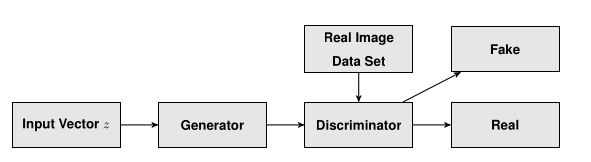
\includegraphics[scale=.45]{gan}
	\caption{GAN}
\end{figure}

\begin{multline*}
\min_G\max_D V(D,G) = E_{x~p_{data}(x)}[log D(x)] \\
+ E_{z~p_z(z)}[log(1 - D(G(z)))].
\end{multline*}

\end{frame}

\begin{frame} % introduction requirement steg

% Requirements for steganography
Requirements for steganography 
	\begin{itemize}
		\item<1-> Imperceptibility 
		\item<2->  Robustness 
		\item<3->  payload capacity 
	\end{itemize}
\end{frame}

\section{Literature Review}
\begin{frame}{Literature Review} % Literature reveiw


% cover synthesis
Different approaches to steganography
\begin{itemize}
	\item cover modification 
	\item cover synthesis: \shortcite{fridrich2009steganography}
\end{itemize}

\end{frame}

\begin{frame} % Literature Gans in stego

% GANs in stego
GAN in Steganography.
\begin{itemize}
	\item <1-> \shortcite{volkhonskiy2017steganographic}
	\item <2-> \shortcite{shi2017ssgan}
	\item <3-> And some more others \shortcite{tang2017automatic},\shortcite{hayes2017generating}
\end{itemize}
\end{frame}

\begin{frame} % Literature Ke
	
	% Ke
	\begin{figure}
		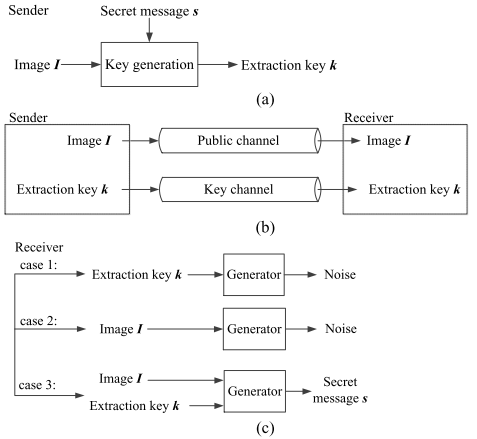
\includegraphics[scale=0.5]{../images/Ke}
		\caption{Proposed System in \shortcite{Ke}}
	\end{figure}
\end{frame}

\begin{frame} % Literature Hu
	% Hu
	\begin{figure}
		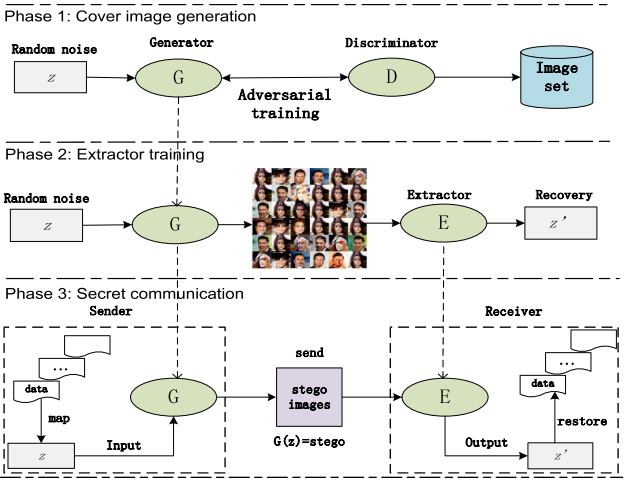
\includegraphics[scale=0.4]{../images/Hu}
		\caption{Proposed System in \cite{Hu2018}}
	\end{figure}
\end{frame}

\begin{frame} % Literature Zhang
	% Zhang
	\begin{figure}
		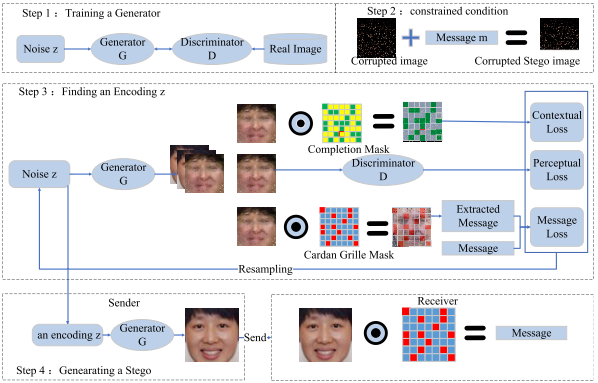
\includegraphics[scale=0.45]{../images/zhang}
		\caption{Proposed System in \shortcite{Zhang2019}}
	\end{figure}
\end{frame}

\section{Problem Statement}
\begin{frame}{Problem Statement} % Problem Statement
	
	% problem statement
	
	Observed problems: 
	\begin{itemize}
		\item Instability of Training
		\item Slow convergence
		\item Inadequately realistic image generation
	\end{itemize}

\pause
\visible{\textbf{\textquotedblleft This is mainly associated to the GAN technique used in the
		framework.\textquotedblright}}

\end{frame}

\section{Objectives}
\begin{frame}{Objectives} % Objective general

	%general objectives
	Design and implement a powerful generative steganographic framework using a
most suitable GAN.
\end{frame}

\begin{frame} %objective specific
	
	%specific objectives
	Specific objectives:
	\begin{itemize}
		\item <1-> Improve stability of Training and convergence speed.
		\item <2-> Generate more realistic image.
		\item <3-> Maintain state of the art security.
	\end{itemize}
	
\end{frame}

\section{Methodology}
\begin{frame}{Methodology} % Methodology architecture

	% system architecture
	\begin{figure}
		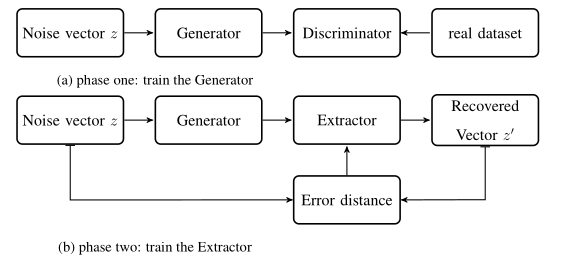
\includegraphics[scale=.45]{arch}
		\caption{System Architecture}
	\end{figure}
\end{frame}

\begin{frame} % Methodology Gan types

	% choice of GAN
	Choice of GAN: 
	\begin{itemize}
		\item BEGAN
		\item RGAN
		\item WGAN-DIV
		\item WGAN-GP
	\end{itemize}
\end{frame}

\begin{frame} % Methodology dataset

 % choice of dataset
 Choice of dataset:
 \begin{itemize}
 	\item CelebA
 	\item LFW
 	\item Food101
 	\item MNIST
 \end{itemize}
\end{frame}

\begin{frame} % Methodology testing method
	
	% testing methods
	Choice of testing method:
	\begin{itemize}
		\item Visual instpection
		\item Inception score
		\item Visual Turing test
		\item MOS
	\end{itemize}
\end{frame}

\section{Scope}
\begin{frame}{Scope} % Scope

\begin{itemize}
	\item <1-> Robustness
	\item <2-> Passive Adversary
	\item <3-> Payload Capacity
	\item <4-> Imperceptibility
\end{itemize}
\end{frame}

\section{Significance Of The Study}
\begin{frame}{Significance Of The Study} % significance

	The main problem in generative steganography 
	
	\begin{center}
		\textbf{Imperceptibility}
	\end{center}
\end{frame}

\section{Work Plan}
\begin{frame}{Work Plan} % Workplan

\begin{figure}
	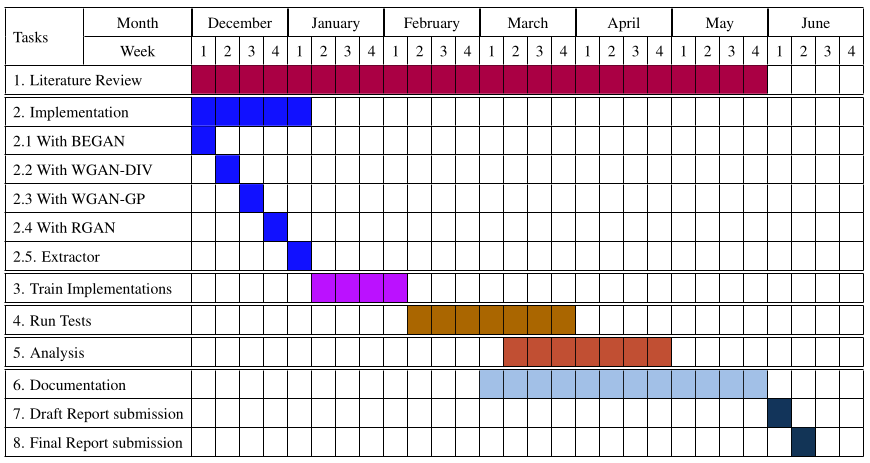
\includegraphics[width=10cm]{../images/workplan}
	\caption{Proposed work plan}
\end{figure}
\end{frame}

\section{Budget}
\begin{frame}{Budget} % Budget

Main cost of the project: 
\begin{itemize}
	\item Powerful GPU for training. 
	\begin{itemize}
		\item From the university
		\item Amazon EC2
		\item Google Cloud
	\end{itemize}
\end{itemize}
\end{frame}

\begin{frame} [allowframebreaks] {Reference}% reference
	
	\bibliographystyle{apacite}
	\bibliography{../bib/reference}
\end{frame}

\begin{frame} % Thank you
\begin{center}
\LARGE
THANK YOU
\end{center}
\end{frame}
\end{document}